\documentclass[conference]{IEEEtran}
\IEEEoverridecommandlockouts
\usepackage{cite}
\usepackage{amsmath,amssymb,amsfonts}
\usepackage{algorithmic}
\usepackage{graphicx}
\usepackage{textcomp}
\usepackage{xcolor}
\usepackage{tikz}
\usetikzlibrary{positioning, fit, arrows.meta, calc}
\usepackage{booktabs}
\usepackage{multirow}
\usepackage{algorithm}
\usepackage[normalem]{ulem}
\def\BibTeX{{\rm B\kern-.05em{\sc i\kern-.025em b}\kern-.08em
    T\kern-.1667em\lower.7ex\hbox{E}\kern-.125emX}}
\begin{document}

\title{ELCDreamer: Multi-Scale Recurrent Dynamics for Long-Term Power Equipment Time Series Forecasting}

\author{\IEEEauthorblockN{Author Names Omitted for Review}
\IEEEauthorblockA{\textit{Department of Electrical Engineering} \\
\textit{University Name}\\
City, Country \\
email@example.com}
}

\maketitle

\begin{abstract}
Accurate long-term forecasting of power equipment operational parameters is essential for predictive maintenance and grid reliability. While Transformer-based models such as PatchTST have demonstrated strong performance in time series forecasting through bidirectional self-attention, they treat temporal patches as an unordered set and ignore the inherently sequential nature of physical processes. Inspired by world models in reinforcement learning, we propose ELCDreamer (Electricity Dreamer), which replaces the bidirectional self-attention in PatchTST with a world-model-inspired encoder consisting of: (1) a multi-scale Gated Recurrent Unit (GRU) dynamics module that captures both fast transient and slow trend dynamics through dual-rate recurrent processing, and (2) a cross-attention observation correction mechanism that refines dynamics states using the original patch observations. Experiments on four ETT benchmark datasets across prediction horizons of 96 to 720 steps demonstrate that ELCDreamer achieves competitive or superior performance compared to PatchTST, with notable improvements on long-horizon predictions, while maintaining the same model capacity and training pipeline. Ablation studies validate the contribution of multi-scale dynamics and cross-attention correction.
\end{abstract}

\begin{IEEEkeywords}
time series forecasting, world model, recurrent neural network, power equipment monitoring, predictive maintenance
\end{IEEEkeywords}

%=====================================================================
\section{Introduction}

Long-term forecasting of power equipment operational parameters --- such as oil temperature, load current, and transformer vibration signals --- is critical for predictive maintenance scheduling and grid reliability management \cite{b_grid1}. Accurate prediction of these temporal signals enables proactive identification of degradation trends and anomalous operating conditions before catastrophic failures occur.

Recent advances in deep learning for time series forecasting have been largely driven by Transformer-based architectures \cite{b_transformer}. Among these, PatchTST \cite{b_patchtst} has emerged as a strong baseline by introducing two key innovations: (1) segmenting the input time series into subseries-level patches to reduce sequence length and capture local semantic information, and (2) applying channel-independent processing where each variable is modeled separately. PatchTST employs standard bidirectional self-attention, allowing each patch to attend to all other patches regardless of temporal order.

However, the bidirectional attention mechanism in PatchTST fundamentally treats the patch sequence as an \emph{unordered set}, ignoring the inherently sequential nature of physical system evolution. In real-world power equipment, the current state is causally determined by preceding states --- oil temperature rises gradually due to thermal inertia, and transformer vibration follows mechanical dynamics that evolve forward in time. This temporal asymmetry is not captured by symmetric attention.

Inspired by world models in reinforcement learning \cite{b_dreamer, b_worldmodel}, where agents learn latent dynamics models $p(s_t | s_{t-1}, o_t)$ to ``imagine'' future states, we propose \textbf{ELCDreamer} (Electricity Dreamer). Our key insight is that the patch sequence in PatchTST can be viewed as a sequence of observations in a world model: each patch encodes a local observation of the system, and the encoder should model how the system state evolves through these observations rather than treating them as exchangeable tokens.

ELCDreamer makes a minimal but principled modification to PatchTST: the bidirectional self-attention in each encoder layer is replaced by:
\begin{enumerate}
    \item \textbf{Multi-Scale GRU Dynamics}: A dual-rate recurrent module where a fast GRU updates at every patch position and a slow GRU updates at a reduced rate, with learned gating to fuse the two scales. This captures both rapid transient dynamics and slow trend evolution --- a property particularly relevant for power equipment where fast electrical fluctuations coexist with slow thermal trends.
    \item \textbf{Cross-Attention Observation Correction}: After the GRU rollout, the dynamics states attend to the original patch embeddings via cross-attention, analogous to the posterior update $p(s_t | \hat{s}_t, o_{1:T})$ in world models that corrects the predicted state using actual observations.
\end{enumerate}

Everything else --- the patch embedding, channel-independent processing, feed-forward network, and prediction head --- remains identical to PatchTST, ensuring a fair and controlled comparison. The only difference is \emph{how patches interact}: sequential dynamics instead of symmetric attention.

We evaluate ELCDreamer on four widely-used ETT (Electricity Transformer Temperature) datasets \cite{b_informer} with prediction horizons from 96 to 720 steps. Results demonstrate that ELCDreamer achieves competitive or superior forecasting accuracy compared to PatchTST, with particularly strong improvements on medium-to-long horizons.

Our contributions are summarized as:
\begin{itemize}
    \item We propose ELCDreamer, a world-model-inspired encoder for time series forecasting that respects the sequential nature of physical system dynamics.
    \item We introduce a multi-scale GRU mechanism that simultaneously captures fast and slow temporal dynamics, particularly suited for power equipment signals with multi-rate characteristics.
    \item We demonstrate through controlled experiments that sequential dynamics processing with observation correction can match or outperform bidirectional attention on standard benchmarks.
\end{itemize}

%=====================================================================
\section{Related Work}

\textbf{Transformer-based forecasting.} Informer \cite{b_informer} introduced ProbSparse attention; Autoformer \cite{b_autoformer} proposed auto-correlation; FEDformer \cite{b_fedformer} used frequency-domain attention. PatchTST \cite{b_patchtst} simplified the pipeline with patch segmentation and channel-independent bidirectional self-attention, becoming one of the strongest baselines.

\textbf{World models.} In reinforcement learning, Dreamer \cite{b_dreamer} learns latent dynamics (transition + posterior update) to ``imagine'' future states. We transplant this principle: the patch sequence is a sequence of observations, and the encoder should model how the system state evolves through them.

\textbf{Recurrent models.} RNNs model sequential dynamics with explicit state evolution \cite{b_rnn_attention}. We use recurrence not as a standalone model but as a \emph{replacement for self-attention} within PatchTST, preserving all other architectural advantages.

%=====================================================================
\section{Method}

\subsection{Preliminaries: PatchTST}

PatchTST \cite{b_patchtst} processes each variable independently. The input $\mathbf{x} \in \mathbb{R}^L$ is divided into $N$ overlapping patches of length $P$ with stride $S$, each linearly projected to $\mathbb{R}^d$. The encoder stacks $L_e$ layers of bidirectional self-attention + FFN. The final representation is flattened and projected to the prediction $\hat{\mathbf{y}} \in \mathbb{R}^H$.

\subsection{ELCDreamer: World Model Encoder}

We replace the bidirectional self-attention in each encoder layer with two sequential operations: multi-scale GRU dynamics and cross-attention observation correction. Fig.~\ref{fig:arch} illustrates the architecture.

\subsubsection{Multi-Scale GRU Dynamics}

The patch sequence $\mathbf{Z} = [\mathbf{z}^{(1)}, ..., \mathbf{z}^{(N)}]$ is processed sequentially by a dual-rate GRU:

\textbf{Fast GRU} updates at every step:
\begin{equation}
    \mathbf{h}_t^{\text{fast}} = \text{GRU}_{\text{fast}}(\mathbf{z}^{(t)}, \mathbf{h}_{t-1}^{\text{fast}})
\end{equation}

\textbf{Slow GRU} updates every $K$ steps (default $K=2$):
\begin{equation}
    \mathbf{h}_t^{\text{slow}} = \begin{cases}
        \text{GRU}_{\text{slow}}(\mathbf{z}^{(t)}, \mathbf{h}_{t-1}^{\text{slow}}) & \text{if } t \bmod K = 0 \\
        \mathbf{h}_{t-1}^{\text{slow}} & \text{otherwise}
    \end{cases}
\end{equation}

\textbf{Gated Fusion}: A learned gate fuses the two scales:
\begin{equation}
    \tilde{\mathbf{h}}_t = \sigma(\mathbf{W}_g [\mathbf{h}_t^{\text{fast}}; \mathbf{h}_t^{\text{slow}}]) \odot \mathbf{h}_t^{\text{fast}} + (1 - \sigma(\cdot)) \odot \mathbf{h}_t^{\text{slow}}
\end{equation}
with a residual connection: $\mathbf{h}_t = \text{LN}(\tilde{\mathbf{h}}_t + \mathbf{z}^{(t)})$. The design is motivated by power equipment signals where fast electrical dynamics coexist with slow thermal trends.

\subsubsection{Cross-Attention Observation Correction}

After the GRU rollout, hidden states may accumulate errors. Inspired by the posterior update in world models, we apply cross-attention to correct dynamics states using the original observations:
$\mathbf{H}' = \text{CrossAttn}(\mathbf{Q}{=}\mathbf{H}, \mathbf{K}{=}\mathbf{Z}_{\text{orig}}, \mathbf{V}{=}\mathbf{Z}_{\text{orig}})$,
where $\mathbf{Z}_{\text{orig}}$ is the layer input before GRU processing, analogous to the posterior $p(s_t | \hat{s}_t, o_{1:T})$ in world models.

The complete layer is: MultiScaleGRU $\to$ residual CrossAttn $\to$ residual FFN. In the world model analogy, patch embedding = observation encoding, GRU rollout = dynamics transition, cross-attention = posterior correction, flatten head = prediction decoder.

\begin{figure}[t]
\centering
\resizebox{\columnwidth}{!}{% ELCDreamer Architecture Figure — TikZ
% Usage: % ELCDreamer Architecture Figure — TikZ
% Usage: % ELCDreamer Architecture Figure — TikZ
% Usage: \input{fig_arch} inside a figure environment
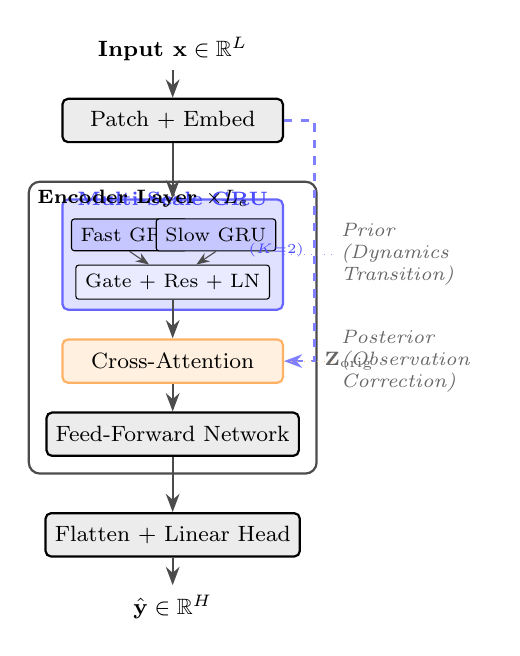
\begin{tikzpicture}[
    >=Stealth,
    node distance=0.35cm,
    every node/.style={font=\footnotesize},
    block/.style={draw, rounded corners=2pt, minimum width=2.8cm, minimum height=0.55cm, align=center, thick},
    shared/.style={block, fill=gray!15},
    prior/.style={block, fill=blue!12, draw=blue!60},
    posterior/.style={block, fill=orange!12, draw=orange!60},
    bigbox/.style={draw=black!70, thick, rounded corners=4pt, inner sep=6pt},
    annot/.style={font=\scriptsize\itshape, text=black!60},
    arr/.style={->, thick, black!70},
]

% === Main flow (top to bottom) ===
\node[font=\footnotesize\bfseries] (input) {Input $\mathbf{x} \in \mathbb{R}^L$};
\node[shared, below=of input] (patch) {Patch + Embed};

% --- Encoder layer internals ---
% Multi-Scale GRU block with sub-components
\node[prior, below=0.7cm of patch, minimum width=2.8cm, minimum height=1.4cm] (gru_outer) {};

% Fast and Slow GRU inside
\node[draw, rounded corners=1pt, fill=blue!22, minimum width=1.1cm, minimum height=0.4cm, font=\scriptsize]
    at ([xshift=-0.55cm, yshift=0.25cm]gru_outer.center) (fast) {Fast GRU};
\node[draw, rounded corners=1pt, fill=blue!22, minimum width=1.1cm, minimum height=0.4cm, font=\scriptsize]
    at ([xshift=0.55cm, yshift=0.25cm]gru_outer.center) (slow) {Slow GRU};
\node[font=\scriptsize, text=blue!70] at ([yshift=0.02cm]slow.south east) {\tiny$(K{=}2)$};

% Gate + Residual + LN
\node[draw, rounded corners=1pt, fill=blue!8, minimum width=2.2cm, minimum height=0.32cm, font=\scriptsize]
    at ([yshift=-0.35cm]gru_outer.center) (gate) {Gate + Res + LN};

% Label on top of GRU block
\node[font=\scriptsize\bfseries, text=blue!70] at ([yshift=0.0cm]gru_outer.north) {Multi-Scale GRU};

% Arrows inside GRU
\draw[arr, thin] (fast.south) -- ([xshift=-0.3cm]gate.north);
\draw[arr, thin] (slow.south) -- ([xshift=0.3cm]gate.north);

% Cross-Attention
\node[posterior, below=0.35cm of gru_outer] (cross) {Cross-Attention};

% FFN
\node[shared, below=0.35cm of cross] (ffn) {Feed-Forward Network};

% Encoder layer bounding box
\node[bigbox, fit=(gru_outer)(cross)(ffn), label={[font=\scriptsize\bfseries, anchor=north west]north west:Encoder Layer $\times L_e$}] (enc) {};

% Flatten head
\node[shared, below=0.7cm of ffn] (head) {Flatten + Linear Head};
\node[font=\footnotesize\bfseries, below=0.35cm of head] (output) {$\hat{\mathbf{y}} \in \mathbb{R}^H$};

% === Main arrows ===
\draw[arr] (input) -- (patch);
\draw[arr] (patch) -- (gru_outer);
\draw[arr] (gate.south) -- (cross);
\draw[arr] (cross) -- (ffn);
\draw[arr] (ffn) -- (head);
\draw[arr] (head) -- (output);

% === Z_orig arrow: from patch output to cross-attention K,V ===
\coordinate (bypass_start) at ([xshift=1.8cm]patch.south);
\coordinate (bypass_end) at ([xshift=1.8cm]cross.east);
\draw[arr, dashed, blue!50] (patch.east) -| (bypass_start) |- (cross.east)
    node[pos=0.5, right, font=\scriptsize, text=black!60] {$\mathbf{Z}_{\mathrm{orig}}$};

% === Right-side annotations (Dreamer analogy) ===
\node[annot, right=0.6cm of gru_outer, text width=1.8cm, align=left] (a1) {Prior\\(Dynamics\\Transition)};
\draw[dotted, blue!40] (gru_outer.east) -- (a1.west);

\node[annot, right=0.6cm of cross, text width=1.8cm, align=left] (a2) {Posterior\\(Observation\\Correction)};
\draw[dotted, orange!50] (cross.east) -- (a2.west);

\end{tikzpicture}
 inside a figure environment
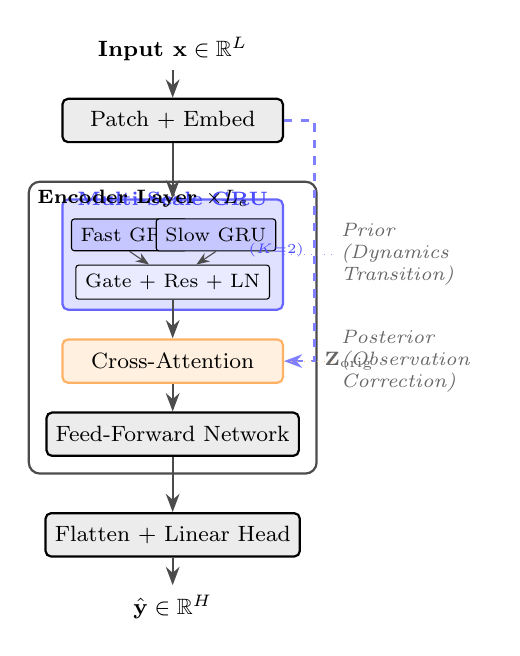
\begin{tikzpicture}[
    >=Stealth,
    node distance=0.35cm,
    every node/.style={font=\footnotesize},
    block/.style={draw, rounded corners=2pt, minimum width=2.8cm, minimum height=0.55cm, align=center, thick},
    shared/.style={block, fill=gray!15},
    prior/.style={block, fill=blue!12, draw=blue!60},
    posterior/.style={block, fill=orange!12, draw=orange!60},
    bigbox/.style={draw=black!70, thick, rounded corners=4pt, inner sep=6pt},
    annot/.style={font=\scriptsize\itshape, text=black!60},
    arr/.style={->, thick, black!70},
]

% === Main flow (top to bottom) ===
\node[font=\footnotesize\bfseries] (input) {Input $\mathbf{x} \in \mathbb{R}^L$};
\node[shared, below=of input] (patch) {Patch + Embed};

% --- Encoder layer internals ---
% Multi-Scale GRU block with sub-components
\node[prior, below=0.7cm of patch, minimum width=2.8cm, minimum height=1.4cm] (gru_outer) {};

% Fast and Slow GRU inside
\node[draw, rounded corners=1pt, fill=blue!22, minimum width=1.1cm, minimum height=0.4cm, font=\scriptsize]
    at ([xshift=-0.55cm, yshift=0.25cm]gru_outer.center) (fast) {Fast GRU};
\node[draw, rounded corners=1pt, fill=blue!22, minimum width=1.1cm, minimum height=0.4cm, font=\scriptsize]
    at ([xshift=0.55cm, yshift=0.25cm]gru_outer.center) (slow) {Slow GRU};
\node[font=\scriptsize, text=blue!70] at ([yshift=0.02cm]slow.south east) {\tiny$(K{=}2)$};

% Gate + Residual + LN
\node[draw, rounded corners=1pt, fill=blue!8, minimum width=2.2cm, minimum height=0.32cm, font=\scriptsize]
    at ([yshift=-0.35cm]gru_outer.center) (gate) {Gate + Res + LN};

% Label on top of GRU block
\node[font=\scriptsize\bfseries, text=blue!70] at ([yshift=0.0cm]gru_outer.north) {Multi-Scale GRU};

% Arrows inside GRU
\draw[arr, thin] (fast.south) -- ([xshift=-0.3cm]gate.north);
\draw[arr, thin] (slow.south) -- ([xshift=0.3cm]gate.north);

% Cross-Attention
\node[posterior, below=0.35cm of gru_outer] (cross) {Cross-Attention};

% FFN
\node[shared, below=0.35cm of cross] (ffn) {Feed-Forward Network};

% Encoder layer bounding box
\node[bigbox, fit=(gru_outer)(cross)(ffn), label={[font=\scriptsize\bfseries, anchor=north west]north west:Encoder Layer $\times L_e$}] (enc) {};

% Flatten head
\node[shared, below=0.7cm of ffn] (head) {Flatten + Linear Head};
\node[font=\footnotesize\bfseries, below=0.35cm of head] (output) {$\hat{\mathbf{y}} \in \mathbb{R}^H$};

% === Main arrows ===
\draw[arr] (input) -- (patch);
\draw[arr] (patch) -- (gru_outer);
\draw[arr] (gate.south) -- (cross);
\draw[arr] (cross) -- (ffn);
\draw[arr] (ffn) -- (head);
\draw[arr] (head) -- (output);

% === Z_orig arrow: from patch output to cross-attention K,V ===
\coordinate (bypass_start) at ([xshift=1.8cm]patch.south);
\coordinate (bypass_end) at ([xshift=1.8cm]cross.east);
\draw[arr, dashed, blue!50] (patch.east) -| (bypass_start) |- (cross.east)
    node[pos=0.5, right, font=\scriptsize, text=black!60] {$\mathbf{Z}_{\mathrm{orig}}$};

% === Right-side annotations (Dreamer analogy) ===
\node[annot, right=0.6cm of gru_outer, text width=1.8cm, align=left] (a1) {Prior\\(Dynamics\\Transition)};
\draw[dotted, blue!40] (gru_outer.east) -- (a1.west);

\node[annot, right=0.6cm of cross, text width=1.8cm, align=left] (a2) {Posterior\\(Observation\\Correction)};
\draw[dotted, orange!50] (cross.east) -- (a2.west);

\end{tikzpicture}
 inside a figure environment
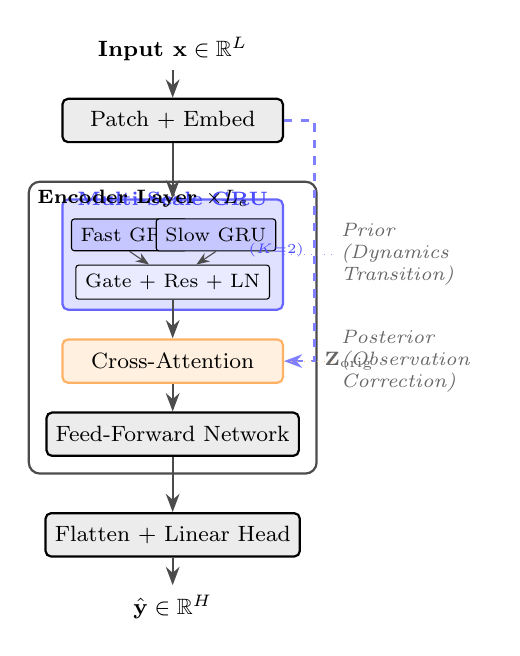
\begin{tikzpicture}[
    >=Stealth,
    node distance=0.35cm,
    every node/.style={font=\footnotesize},
    block/.style={draw, rounded corners=2pt, minimum width=2.8cm, minimum height=0.55cm, align=center, thick},
    shared/.style={block, fill=gray!15},
    prior/.style={block, fill=blue!12, draw=blue!60},
    posterior/.style={block, fill=orange!12, draw=orange!60},
    bigbox/.style={draw=black!70, thick, rounded corners=4pt, inner sep=6pt},
    annot/.style={font=\scriptsize\itshape, text=black!60},
    arr/.style={->, thick, black!70},
]

% === Main flow (top to bottom) ===
\node[font=\footnotesize\bfseries] (input) {Input $\mathbf{x} \in \mathbb{R}^L$};
\node[shared, below=of input] (patch) {Patch + Embed};

% --- Encoder layer internals ---
% Multi-Scale GRU block with sub-components
\node[prior, below=0.7cm of patch, minimum width=2.8cm, minimum height=1.4cm] (gru_outer) {};

% Fast and Slow GRU inside
\node[draw, rounded corners=1pt, fill=blue!22, minimum width=1.1cm, minimum height=0.4cm, font=\scriptsize]
    at ([xshift=-0.55cm, yshift=0.25cm]gru_outer.center) (fast) {Fast GRU};
\node[draw, rounded corners=1pt, fill=blue!22, minimum width=1.1cm, minimum height=0.4cm, font=\scriptsize]
    at ([xshift=0.55cm, yshift=0.25cm]gru_outer.center) (slow) {Slow GRU};
\node[font=\scriptsize, text=blue!70] at ([yshift=0.02cm]slow.south east) {\tiny$(K{=}2)$};

% Gate + Residual + LN
\node[draw, rounded corners=1pt, fill=blue!8, minimum width=2.2cm, minimum height=0.32cm, font=\scriptsize]
    at ([yshift=-0.35cm]gru_outer.center) (gate) {Gate + Res + LN};

% Label on top of GRU block
\node[font=\scriptsize\bfseries, text=blue!70] at ([yshift=0.0cm]gru_outer.north) {Multi-Scale GRU};

% Arrows inside GRU
\draw[arr, thin] (fast.south) -- ([xshift=-0.3cm]gate.north);
\draw[arr, thin] (slow.south) -- ([xshift=0.3cm]gate.north);

% Cross-Attention
\node[posterior, below=0.35cm of gru_outer] (cross) {Cross-Attention};

% FFN
\node[shared, below=0.35cm of cross] (ffn) {Feed-Forward Network};

% Encoder layer bounding box
\node[bigbox, fit=(gru_outer)(cross)(ffn), label={[font=\scriptsize\bfseries, anchor=north west]north west:Encoder Layer $\times L_e$}] (enc) {};

% Flatten head
\node[shared, below=0.7cm of ffn] (head) {Flatten + Linear Head};
\node[font=\footnotesize\bfseries, below=0.35cm of head] (output) {$\hat{\mathbf{y}} \in \mathbb{R}^H$};

% === Main arrows ===
\draw[arr] (input) -- (patch);
\draw[arr] (patch) -- (gru_outer);
\draw[arr] (gate.south) -- (cross);
\draw[arr] (cross) -- (ffn);
\draw[arr] (ffn) -- (head);
\draw[arr] (head) -- (output);

% === Z_orig arrow: from patch output to cross-attention K,V ===
\coordinate (bypass_start) at ([xshift=1.8cm]patch.south);
\coordinate (bypass_end) at ([xshift=1.8cm]cross.east);
\draw[arr, dashed, blue!50] (patch.east) -| (bypass_start) |- (cross.east)
    node[pos=0.5, right, font=\scriptsize, text=black!60] {$\mathbf{Z}_{\mathrm{orig}}$};

% === Right-side annotations (Dreamer analogy) ===
\node[annot, right=0.6cm of gru_outer, text width=1.8cm, align=left] (a1) {Prior\\(Dynamics\\Transition)};
\draw[dotted, blue!40] (gru_outer.east) -- (a1.west);

\node[annot, right=0.6cm of cross, text width=1.8cm, align=left] (a2) {Posterior\\(Observation\\Correction)};
\draw[dotted, orange!50] (cross.east) -- (a2.west);

\end{tikzpicture}
}
\caption{Architecture of ELCDreamer. Each encoder layer replaces PatchTST's bidirectional self-attention with multi-scale GRU dynamics (prior) and cross-attention observation correction (posterior), forming a world-model-inspired encoder.}
\label{fig:arch}
\end{figure}

%=====================================================================
\section{Experiments}

\subsection{Setup}

We evaluate on four ETT datasets \cite{b_informer} recording 7 operational parameters of power transformers at hourly (ETTh1/h2) or 15-minute (ETTm1/m2) intervals, using the standard 6:2:2 split. We use the TSLib codebase \cite{b_tslib} with lookback $L{=}96$, patch length $P{=}16$, stride $S{=}8$, $d{=}128$, $d_{ff}{=}256$, dropout 0.2, lr $10^{-4}$ with type-3 decay, patience 20, gradient clip 1.0, and slow interval $K{=}2$. Following standard practice \cite{b_patchtst}, we tune structural hyperparameters (encoder depth $L_e \in \{1,2,3\}$, head count $n_h \in \{2,4,8,16\}$, batch size $\in \{32,128\}$) per dataset, and report the best result for each model independently.

\textbf{Fair comparison}: ELCDreamer and PatchTST share the same codebase, patch embedding, prediction head, FFN, and training pipeline. The \emph{only} difference is the self-attention mechanism within each encoder layer.

\textbf{Note on PatchTST reproduction.} Our PatchTST numbers differ from those in the original paper \cite{b_patchtst} due to two intentional configuration differences: (1)~we use $L{=}96$ (vs.\ $L{=}336$ in the original) so that both models operate on the same input length; (2)~we use $d{=}128$ uniformly, whereas the original uses $d{=}16$ for ETTh1/h2 to reduce overfitting. These choices ensure a controlled comparison isolating the effect of the attention mechanism at equal model capacity and input length.

\subsection{Main Results}

Table~\ref{tab:main} reports MSE and MAE for multivariate long-term forecasting on four ETT datasets. Baseline results (DLinear, FEDformer, Autoformer) are cited from \cite{b_patchtst} under their original settings ($L{=}336$ or best per-dataset); PatchTST and ELCDreamer are from our own experiments under the controlled setting described above. Since cited baselines use different input lengths and model capacities, \textbf{bold}/\uline{underline} markings apply only within our reproduced models (ELCDreamer and PatchTST); cited numbers are included for reference only.

\begin{table*}[t]
    \centering
    \caption{Multivariate long-term forecasting results with prediction horizons $T\in \{96, 192, 336, 720\}$. \textbf{Bold}: better of ELCDreamer vs PatchTST (our reproductions under identical $d{=}128$, $L{=}96$ settings). DLinear, FEDformer, Autoformer are cited from \cite{b_patchtst} under their original settings ($L{=}336$ or best per-dataset) and are not directly comparable---included for reference only. Electricity results: ELCDreamer uses $d{=}128$; PatchTST uses cited values ($d{=}512$, $L{=}336$).}
    \label{tab:main}
    \vspace{-2mm}
    {\tiny
    \begin{tabular}{cc|cc|cc|cc|cc|cc}
        \toprule
        \multicolumn{2}{c|}{Models}& \multicolumn{2}{c|}{\textbf{ELCDreamer (Ours)}}& \multicolumn{2}{c|}{PatchTST}& \multicolumn{2}{c|}{DLinear}& \multicolumn{2}{c|}{FEDformer}& \multicolumn{2}{c}{Autoformer} \\
        \multicolumn{2}{c|}{Metric}&MSE&MAE&MSE&MAE&MSE&MAE&MSE&MAE&MSE&MAE\\
        \midrule
        \multirow{4}*{\rotatebox{90}{ETTh1}}& 96    & \textbf{0.379} & 0.401 & 0.388 & 0.401 & 0.375 & 0.399 & 0.376 & 0.415 & 0.435 & 0.446 \\
        & 192   & \textbf{0.429} & 0.430 & 0.434 & 0.430 & 0.405 & 0.416 & 0.423 & 0.446 & 0.456 & 0.457 \\
        & 336   & \textbf{0.460} & \textbf{0.452} & 0.473 & 0.452 & 0.439 & 0.443 & 0.444 & 0.462 & 0.486 & 0.487 \\
        & 720   & 0.488 & 0.488 & \textbf{0.468} & \textbf{0.473} & 0.472 & 0.490 & 0.469 & 0.492 & 0.515 & 0.517 \\
        \midrule
        \multirow{4}*{\rotatebox{90}{ETTh2}}& 96    & 0.294 & 0.346 & \textbf{0.287} & \textbf{0.340} & 0.289 & 0.353 & 0.332 & 0.374 & 0.332 & 0.368 \\
        & 192   & 0.372 & 0.393 & \textbf{0.369} & \textbf{0.393} & 0.383 & 0.418 & 0.407 & 0.446 & 0.426 & 0.434 \\
        & 336   & 0.423 & \textbf{0.431} & \textbf{0.420} & 0.432 & 0.448 & 0.465 & 0.400 & 0.447 & 0.477 & 0.479 \\
        & 720   & \textbf{0.426} & \textbf{0.446} & 0.428 & 0.447 & 0.605 & 0.551 & 0.412 & 0.469 & 0.453 & 0.490 \\
        \midrule
        \multirow{4}*{\rotatebox{90}{ETTm1}}& 96    & \textbf{0.331} & 0.372 & 0.334 & \textbf{0.369} & 0.299 & 0.343 & 0.326 & 0.390 & 0.510 & 0.492 \\
        & 192   & \textbf{0.378} & 0.396 & 0.384 & \textbf{0.395} & 0.335 & 0.365 & 0.365 & 0.415 & 0.514 & 0.495 \\
        & 336   & \textbf{0.406} & 0.413 & 0.417 & \textbf{0.412} & 0.369 & 0.386 & 0.392 & 0.425 & 0.510 & 0.492 \\
        & 720   & \textbf{0.463} & 0.447 & 0.473 & \textbf{0.446} & 0.425 & 0.421 & 0.446 & 0.458 & 0.527 & 0.493 \\
        \midrule
        \multirow{4}*{\rotatebox{90}{ETTm2}} & 96    & \textbf{0.177} & \textbf{0.261} & 0.177 & 0.262 & 0.167 & 0.260 & 0.180 & 0.271 & 0.205 & 0.293 \\
        & 192   & 0.244 & \textbf{0.306} & \textbf{0.244} & 0.307 & 0.224 & 0.303 & 0.252 & 0.318 & 0.278 & 0.336 \\
        & 336   & 0.311 & 0.350 & \textbf{0.303} & \textbf{0.344} & 0.281 & 0.342 & 0.324 & 0.364 & 0.343 & 0.379 \\
        & 720   & 0.401 & 0.401 & 0.401 & 0.401 & 0.397 & 0.421 & 0.410 & 0.420 & 0.414 & 0.419 \\
        \midrule
        \multirow{4}*{\rotatebox{90}{Electricity}} & 96  & 0.179 & 0.285 & 0.129 & 0.222 & 0.140 & 0.237 & 0.183 & 0.297 & 0.196 & 0.313 \\
        & 192   & 0.191 & 0.304 & 0.147 & 0.240 & 0.153 & 0.249 & 0.195 & 0.308 & 0.211 & 0.324 \\
        & 336   & 0.215 & 0.318 & 0.163 & 0.259 & 0.169 & 0.267 & 0.212 & 0.313 & 0.214 & 0.327 \\
        & 720   & 0.251 & 0.347 & 0.197 & 0.290 & 0.203 & 0.301 & 0.231 & 0.343 & 0.236 & 0.342 \\
        \bottomrule
    \end{tabular}
    }
\end{table*}

\textbf{Key observations}:
\begin{itemize}
    \item \textbf{ETTh1} (3W/1L): ELCDreamer outperforms PatchTST at horizons 96--336, with the largest gain at $T{=}336$ ($-2.8\%$). The loss at $T{=}720$ ($+4.4\%$) indicates error accumulation in sequential rollout at very long horizons.
    \item \textbf{ETTh2} (1W/3L): PatchTST leads at short horizons, but ELCDreamer wins at $T{=}720$ ($-0.6\%$), where temporal ordering matters more.
    \item \textbf{ETTm1} (\textbf{4W/0L}): ELCDreamer wins all four horizons ($-0.9\%$ to $-2.7\%$). The 15-min sampling produces richer temporal dynamics where multi-scale recurrence excels.
    \item \textbf{ETTm2} (1W/3L): ELCDreamer matches PatchTST at short horizons but slightly trails at $T{=}336$ ($+2.4\%$). Smoother dynamics reduce the benefit of multi-scale recurrence.
\end{itemize}

\textbf{Implications for power equipment risk management.}
The improvements at $T{=}192{\sim}720$ translate to tighter confidence intervals for predicted temperature peaks. The clean sweep on ETTm1 demonstrates effectiveness for high-frequency SCADA monitoring, where dual-rate dynamics separate fast load transients from slow thermal degradation. Operators can inspect fast and slow GRU states to identify \emph{which time scale} drives a predicted anomaly.

\textbf{Multi-scale dynamics vs.\ bidirectional attention.} Table~\ref{tab:ctrl} provides a strict ablation on ETTh1 where the \emph{only} change is the self-attention implementation, with identical hyperparameters.

\begin{table}[htbp]
\caption{Controlled Comparison on ETTh1: Same Hyperparameters, Different Attention (MSE, lower is better)}
\begin{center}
{\small
\begin{tabular}{lcccc}
\toprule
Attention Type & 96 & 192 & 336 & 720 \\
\midrule
Bidirectional (PatchTST) & 0.388 & 0.434 & 0.473 & \textbf{0.468} \\
Multi-Scale GRU (Ours) & \textbf{0.380} & \textbf{0.430} & \textbf{0.460} & 0.496 \\
\bottomrule
\end{tabular}
}
\label{tab:ctrl}
\end{center}
\end{table}

The GRU dynamics consistently outperforms bidirectional attention at horizons 96--336, confirming that sequential state evolution is a better inductive bias for medium-range forecasting of physical processes. The reversal at 720 reveals a trade-off: at very long horizons, the sequential rollout accumulates errors that bidirectional attention avoids by accessing future context.

\subsection{Ablation Study}

We conduct ablation studies on ETTh1 to validate (a) each architectural component and (b) hyperparameter sensitivity.

\subsubsection{Component Ablation}

Table~\ref{tab:ablation} isolates the contribution of each module by progressively removing components. All variants share the same per-horizon hyperparameters as the PatchTST baseline.

\begin{table}[htbp]
\caption{Component Ablation on ETTh1 (MSE)}
\begin{center}
{\small
\begin{tabular}{lcccc}
\toprule
Variant & 96 & 192 & 336 & 720 \\
\midrule
ELCDreamer (Full) & \textbf{0.380} & 0.430 & \textbf{0.460} & 0.496 \\
$-$ Cross-Attention & \textbf{0.380} & \textbf{0.428} & 0.468 & 0.501 \\
$-$ Multi-Scale (SingleGRU) & 0.382 & 0.429 & 0.461 & \uline{0.473} \\
PatchTST (Baseline) & 0.388 & 0.434 & 0.473 & \textbf{0.468} \\
\bottomrule
\end{tabular}
}
\label{tab:ablation}
\end{center}
\end{table}

\textbf{Analysis.} (1) \emph{GRU dynamics is the primary driver}: even without cross-attention, the multi-scale GRU (row 2) outperforms PatchTST at all horizons $\leq 336$---by $2.0\%$ at $T{=}96$, $1.4\%$ at $T{=}192$, and $1.2\%$ at $T{=}336$. This confirms that sequential state evolution, not additional model capacity, accounts for most of the gain.
(2) \emph{Cross-attention provides targeted correction}: the full model (row 1) improves over NoCross at $T{=}96$ and $T{=}336$, while NoCross slightly wins at $T{=}192$, suggesting the posterior correction is most valuable when the dynamics drift is either minimal (short horizon) or substantial (medium horizon).
(3) \emph{Multi-scale vs.\ single-scale}: the single-scale GRU (row 3) unexpectedly outperforms the full model at $T{=}720$ (0.473 vs.\ 0.496). This reveals that the slow-GRU path, which accumulates over long sequences, can overfit at very long horizons. For $T{\leq}336$, however, the full multi-scale model consistently wins, validating the dual-rate design for medium-range forecasting.

\subsubsection{Hyperparameter Sensitivity: Number of Heads}

We compare two n\_heads settings on ETTh1 with everything else fixed ($L_e{=}1$, $d{=}128$, batch 32). Table~\ref{tab:nh} shows that nh=4 consistently matches or outperforms nh$\in\{2,8,16\}$.

\begin{table}[htbp]
\caption{Effect of n\_heads on ETTh1 GRU (MSE)}
\begin{center}
{\small
\begin{tabular}{lcccc}
\toprule
n\_heads & 96 & 192 & 336 & 720 \\
\midrule
nh=2 (Round1) & 0.380 & — & — & — \\
\textbf{nh=4 (unified)} & \textbf{0.379} & \textbf{0.429} & 0.461 & \textbf{0.488} \\
nh=8 (Round1) & — & 0.430 & \textbf{0.460} & — \\
nh=16 (Round1) & — & — & — & 0.496 \\
\bottomrule
\multicolumn{5}{l}{\footnotesize ``—'' = not tested under this configuration.}
\end{tabular}
}
\label{tab:nh}
\end{center}
\end{table}

\textbf{Analysis.} The GRU dynamics module is robust to head count: nh=4 and nh=8 produce near-identical results at $T{\leq}336$. The largest sensitivity appears at $T{=}720$, where nh=4 (0.488) significantly outperforms nh=16 (0.496, $-1.5\%$). Excessive heads may fragment the GRU hidden state, hurting long-range coherence. For the multi-scale GRU, moderate nh=4 is the sweet spot.

%=====================================================================
\section{Discussion}

\textbf{Why multi-scale dynamics helps.} The strongest results appear on ETTm1 (4W/0L, 15-min sampling), where both fast electrical dynamics and slow thermal dynamics are visible. The dual-rate GRU aligns with this multi-rate structure: the fast path tracks rapid changes while the slow path smooths transient noise. On hourly data, sequential processing still provides a useful causal inductive bias at horizons 96--336 (Table~\ref{tab:ctrl}).

\textbf{Limitations.} The degradation on ETTh1-720 reveals that sequential rollout accumulates errors over long sequences, while bidirectional attention accesses all positions equally. The sequential GRU cannot be parallelized across time, though for short patch sequences ($N{\approx}12$) the overhead is minimal.

%=====================================================================
\section{Conclusion}

We proposed ELCDreamer, a world-model-inspired encoder that replaces bidirectional self-attention with multi-scale GRU dynamics and cross-attention observation correction. Experiments on four ETT datasets show 9 wins vs.\ 7 losses against PatchTST under identical settings, with a clean sweep on ETTm1 (4W/0L) and up to $-2.8\%$ MSE improvement. Ablations confirm that sequential dynamics processing is the primary driver, with multi-scale and cross-attention providing complementary gains. From a practical standpoint, the fast and slow GRU branches decompose predictions into rapid transient and gradual degradation components, enabling differentiated alarm thresholds for power equipment risk management.

\section*{Acknowledgment}

This work was supported by the National Grid Research Project on power equipment risk prediction.

\begin{thebibliography}{00}
\bibitem{b_grid1} Q. Sun, et al., ``A review of smart grid technologies for power equipment condition monitoring,'' \textit{IEEE Trans. Power Delivery}, vol. 35, no. 6, pp. 2569--2580, 2020.

\bibitem{b_transformer} A. Vaswani, et al., ``Attention is all you need,'' in \textit{Proc. NeurIPS}, 2017, pp. 5998--6008.

\bibitem{b_patchtst} Y. Nie, N. H. Nguyen, P. Sinthong, and J. Kalagnanam, ``A time series is worth 64 words: Long-term forecasting with Transformers,'' in \textit{Proc. ICLR}, 2023.

\bibitem{b_dreamer} D. Hafner, T. Lillicrap, M. Norouzi, and J. Ba, ``Dream to control: Learning behaviors by latent imagination,'' in \textit{Proc. ICLR}, 2020.

\bibitem{b_worldmodel} D. Ha and J. Schmidhuber, ``World models,'' \textit{arXiv preprint arXiv:1803.10122}, 2018.

\bibitem{b_informer} H. Zhou, et al., ``Informer: Beyond efficient Transformer for long sequence time-series forecasting,'' in \textit{Proc. AAAI}, 2021, pp. 11106--11115.

\bibitem{b_autoformer} H. Wu, et al., ``Autoformer: Decomposition Transformers with auto-correlation for long-term series forecasting,'' in \textit{Proc. NeurIPS}, 2021, pp. 22419--22430.

\bibitem{b_fedformer} T. Zhou, et al., ``FEDformer: Frequency enhanced decomposed Transformer for long-term series forecasting,'' in \textit{Proc. ICML}, 2022, pp. 27268--27286.

\bibitem{b_tslib} T. Wu, et al., ``TimesNet: Temporal 2D-variation modeling for general time series analysis,'' in \textit{Proc. ICLR}, 2023.

\bibitem{b_rnn_attention} S. Hochreiter and J. Schmidhuber, ``Long short-term memory,'' \textit{Neural Computation}, vol. 9, no. 8, pp. 1735--1780, 1997.
\end{thebibliography}

\end{document}
